\chapter{Empirical Study}\label{chapter:EmpiricalStudy}
Based on five research questions, a comprehensive empirical study 
was conducted to gain a better understanding of the 
capabilities and constraints of MLLMs in generating accessible UI code.
% To better understand the capabilities and limitations of 
% MLLMs in generating accessible UI code, a comprehensive 
% study guided by four research questions was conducted. 
The following presents the study setup and the quantitative and
qualitative results.

\section{RQ1: Do MLLMs generate accessible code from UI screenshots?}
\subsection{Experiment Setup}
To evaluate the baseline capability of MLLMs in generating accessible
code from visual UI input, two widely-used MLLMs are 
selected for this study: \textit{GPT-4o} and \textit{Gemini-2.0 Flash}.
These models show strong performance in 
multimodal tasks, and their support for image inputs makes
them suitable candidates for this study.\newline
As described in section~\ref{chapter:Methodology}, the models are 
prompted with our dataset of UI screenshots and a corresponding 
task description. The task description includes a naive (plain)
prompt, which instructs the model to generate HTML/CSS code
based on the provided screenshot, without mentioning accessibility.

\newmdenv[
  backgroundcolor=lightgray,
  linecolor=black,
  linewidth=0.5pt,
%   roundcorner=20pt,
  innertopmargin=3pt,
  innerbottommargin=3pt,
  innerleftmargin=10pt,
  innerrightmargin=10pt,
  skipbelow=3pt,
  skipabove=3pt,
]{roundedbox}

\begin{roundedbox}
\textbf{Naive Prompt}: Your task is to replicate 
the provided UI screenshot of a webpage pixel-perfectly using 
HTML/CSS.
\end{roundedbox}

This setup allows to observe whether MLLMs can 
naturally produce accessible code without direct instruction 
and acts as a benchmark for enhancement strategies. 
It is important to note that each experiment is conducted three 
times for each model, and the results below represent the average 
outcomes to account for stochastic fluctuations in the model's responses.


\subsection{Results}
Both models show a strong performance in reconstructing the given 
UI layouts with an average of 88.96\% in code similarity
for GPT and 87.12\% for Gemini, as shown in Table~\ref{tab:table-performance}.
These results demonstrate that the models are capable of generating 
valid and visually similar HTML/CSS code from UI screenshots. 
While a more detailed evaluation of the visual fidelity is beyond 
the scope of this thesis, these results serve as a baseline 
for subsequent accessibility analysis.
Table~\ref{tab:table-performance} presents the number of accessibility 
violations in UI code generated by GPT and Gemini. Despite 
achieving high layout and structural fidelity, both models produce 
a significant amount of accessibility issues. On average, GPT 
generates 13.75 violations per UI, while Gemini produces 15.45, or 12.4\% 
more. The IR is 12.22\% for GPT and 11.42\% for Gemini,
while IWIR is 47.10\% and 47.70\%, respectively. Although Gemini yields
more total violations than GPT on average, an analysis of its DOM size 
reveals that it generates larger code snippets, which explains
its lower IR because the violations are distributed over a larger 
number of nodes. However, the IWIR stays consistent across the two models, 
suggesting that the severity of the violations is similar.
These findings demonstrate a clear gap between visual correctness and 
accessibility compliance and highlight that without clear and 
explicit instructions, MLLMs might not be able to follow 
accessibility principles in code generation. To understand 
the underlying reasons for these accessibility issues, a manual 
analysis of the violations observed in the generated output
has been conducted. This process makes it possible to identify recurring 
failure patterns and model limitations.

\begin{figure}
  \centering
  % \includegraphics[width=0.8\linewidth]{images/common.png}
  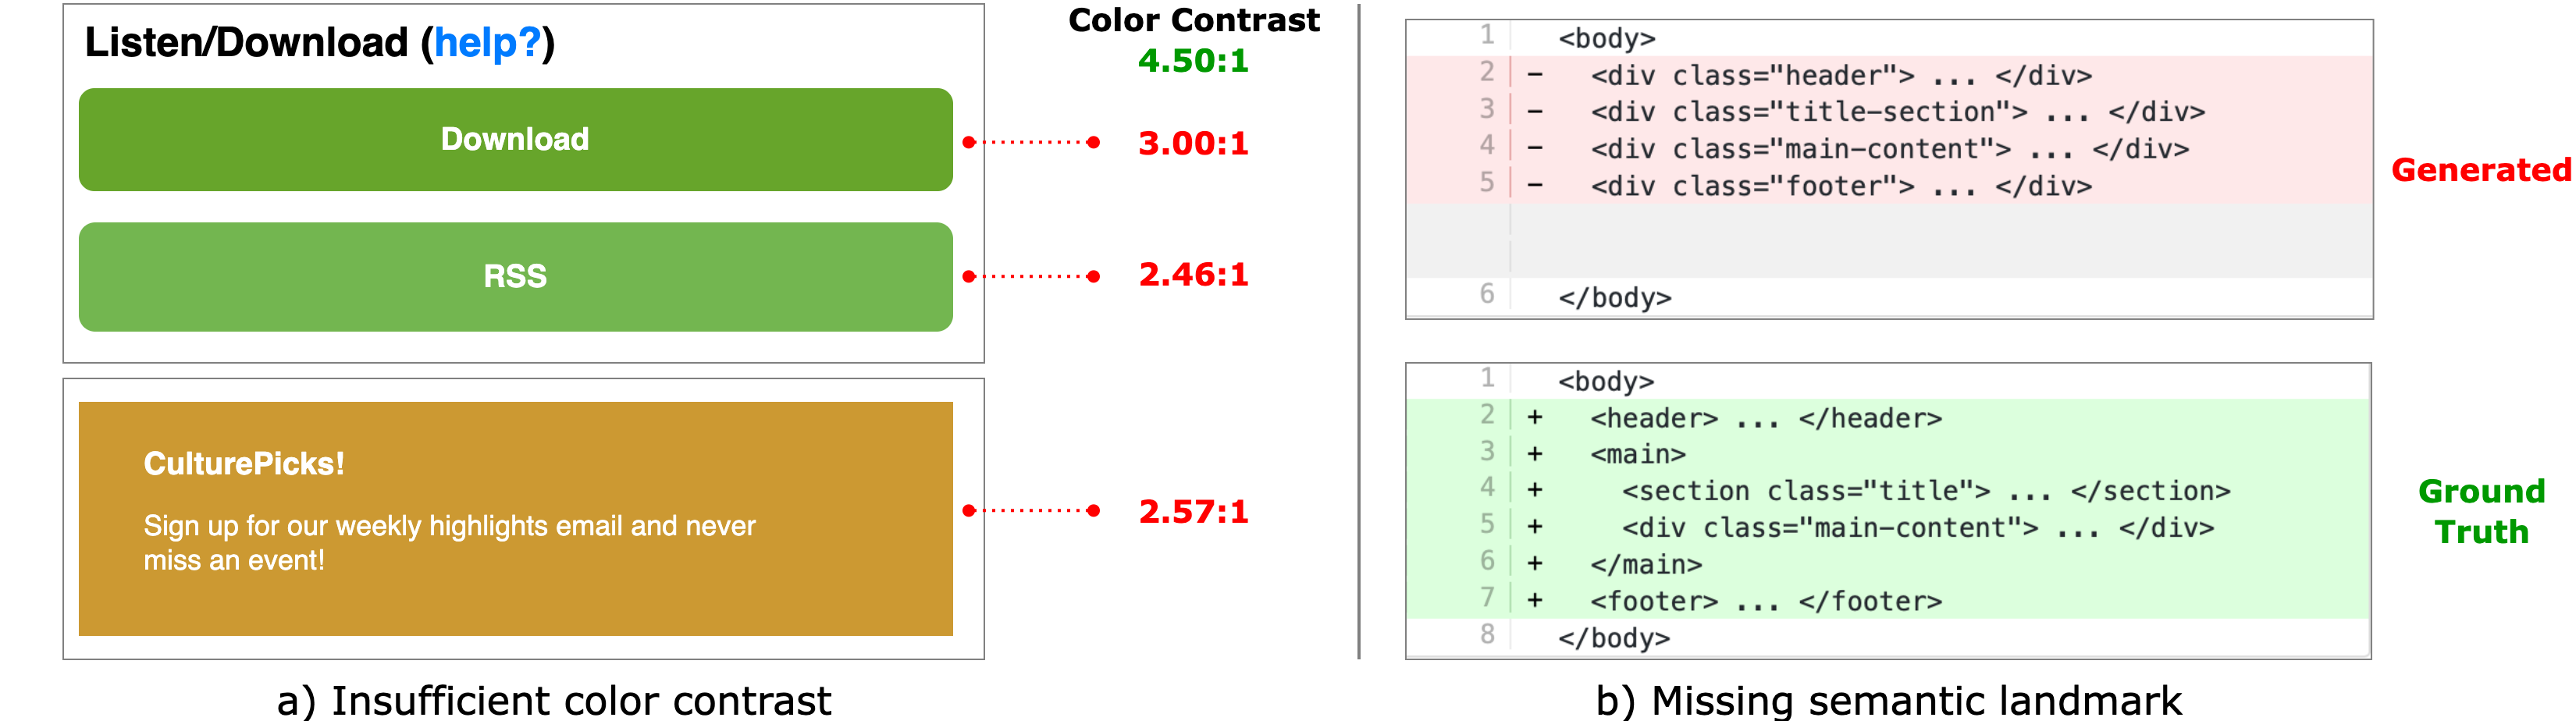
\includegraphics[width=0.9\linewidth]{figures/colorcontrastlandmarkexample.png}
  \caption{Example of common accessibility violations.}
  \label{fig:common} 
\end{figure}

\subsubsection{Most common violations}
The detailed analysis reveals that two primary categories of accessibility
issues are dominant in the generated code across both models.
The first category is insufficient color contrast. For instance,
color contrast violations are very common, causing 5.21 violations 
per UI for GPT and 6.89 for Gemini. The reason for this frequency 
can be attributed to the complexity of contrast checking, which 
requires the model to reason mathematically about RGB or hex values
and their luminance for the human eye, as defined by WCAG. This mathematical 
requirement is not only challenging for MLLMs, but also human 
developers often rely on automated tools to ensure compliance 
in this area. The main difficulty lies in the fact that 
even slight deviations in color selection can lead to significant 
usability barriers for visually impaired users. As shown in 
Figure~\ref{fig:common} (a), the generated code uses white text 
(\#ffffff) on a green background (\#67a52a and \#72b650)
or on a yellow background (\#cc9933). This results in 
contrast ratios of 3.00, 2.46, and 2.57, significantly below the
WCAG 2.1 minimum color contrast threshold of 4.5 for normal text.
Even though this mathematical task is within the capabilities of 
MLLMs, it remains a common challenge across both models because 
of their limited visual-perceptual understanding and mathematical 
precision.\newline
The second category is the lack or incorrect usage of semantic 
landmarks. To convert 
the visual structure of a webpage into a format that
assistive technologies can use, semantic landmarks, 
such as \texttt{<main>}, \texttt{<nav>},
\texttt{<header>}, and \texttt{<footer>}, are essential. 
However, these landmarks are not visually 
displayed in the UI and have no specific representation, making it 
difficult for MLLMs, which rely only on screenshot input,
to identify and generate them correctly. As 
shown in Figure~\ref{fig:common} (b), rather than using 
semantic landmarks, the model substitutes them with 
generic \texttt{<div>} elements. As a result, assistive technologies 
interpret the webpage as a flat structure, without navigational 
and structural details, which are necessary for keyboard users or 
screen reader navigation. This can significantly hinder 
accessibility, especially for users who rely on 
semantic segmentation to jump between regions of a webpage. 
% Essentially, the problem arises, first, due to the absence 
% of visible indicators, second, because of the model’s 
% limited exposure to the underlying meaning of UI 
% elements—the type of information human designers tend 
% to acquire through accessibility trainings or work experience.
The issue basically stems from two factors: first, the lack of 
visible indicators, and second, the model’s limited exposure to 
the underlying meaning of UI elements, which is the type of 
information that human designers often gain from accessibility training or work experience.



\begin{center}
\begin{tcolorbox}[colback=black!5!white,colframe=black!75!black,bottom=-0.05pt,top=-0.05pt]
\textit{\textbf{Finding:}} Even though both GPT and Gemini achieve high layout fidelity, 
they consistently generate code with accessibility violations, 
especially in color contrast and missing landmarks. This indicates 
a fundamental gap between visual accuracy and accessibility compliance.
\end{tcolorbox}
\end{center}


\begingroup
    \renewcommand{\arraystretch}{1.1}
\begin{table}
\tabcolsep=0.5cm
\centering
\small

\begin{tabular}{l|c|c|c|c} 
\hline
\rowcolor{lightgray} \textbf{Violations} & \textbf{GPT} & \textbf{Gemini} & \textbf{Qwen} & \textbf{Llava}  \\ 
\hline
Color contrast & 276 & 365 & 159 & 67 \\
\hline
Landmark \& Region & 279 & 265 & 114 & 187 \\
\hline
Label & 102 & 105 & 21 & 14 \\
\hline
Headings & 26 & 18 & 20 & 17 \\
\hline
Target Size & 15 & 13 & 10 & 15 \\
\hline
Distinguishable Links & 20 & 23 & 2 & 0 \\
\hline
Document Language & 0 & 11 & 0 & 0 \\
\hline
Table Headers & 1 & 7 & 1 & 0 \\
\hline
Incomplete Links & 0 & 4 & 0 & 6 \\
\hline
Image Alt-Text & 4 & 5 & 0 & 1 \\
\hline
\hline
\textbf{Total Violations} & 729 & 819 & 329 & 307 \\
\hline
\textbf{Average Violations} & 13.75 & 15.45 & 6.21 & 5.79 \\
\hline
\textbf{IR} & 12.22\% & 11.42\% & 10.70\% & 12.14\% \\
\hline
\textbf{IWIR} & 47.10\% & 47.70\% & 40.25\% & 40.40\% \\
\hline
\textbf{CodeSim} & 88.96\% & 87.12\% & 70.36\% & 50.50\% \\
\hline
\end{tabular}
\caption{Quantitative comparison of accessibility performance metrics across GPT-4o, Gemini-2.0 Flash, Qwen2.5-VL-7B, and Llava-7B.}
\label{tab:table-performance}
\end{table}
\endgroup


\section{RQ2: Do different MLLMs vary in their ability to generate accessible UI code?}
\subsection{Experiment Setup}
To understand how the choice of MLLMs influences the generation of 
accessible HTML/CSS, the analysis is extended beyond the two 
closed-sourced models used in RQ1. This included two additional 
open-source models, \textit{Qwen2.5-VL-7B} and \textit{Llava-7B}, 
selected for their strong performance in multimodal tasks and 
wide adoption in the research community. 
The 7B parameter variations are used to capture substantial 
differences in model behavior and performance while ensuring 
the feasibility under constrained computational resources and 
reproducibility by other researchers.
Similar to RQ1, all models are prompted with the same 
benchmark dataset and naive prompt,
which instructs the models to generate HTML/CSS from UI screenshots
without referencing accessibility. This setup allows a 
direct comparison across the models.

\subsection{Results}
Table~\ref{tab:table-performance} presents the average 
number of accessibility violations per UI, the IR, IWIR, and 
CodeSim for each model. Surprisingly, the open-source models
Qwen and Llava have the fewest violations, averaging 
6.21 and 5.79 violations per UI. Also, most of the other metrics 
show that these models perform better than the closed-source
models: the average values for the IR are 10.70\% for Qwen and
12.14\% for Llava, while the IWIR is 40.25\%
and 40.40\%, respectively.
Since these results 
are significantly lower than the results of GPT and Gemini, 
a closer analysis was conducted, and three key factors 
influencing the accessibility results were identified: 
training data biases, instructional alignments, and 
code generation capabilities.

\subsubsection{Training Data Biases.} Even if the 
internal training data of closed-source models is not publicly 
available, this qualitative analysis reveals noticeable differences 
in the models' behavior that can be attributed to training 
data biases.\newline
The first visible difference is the tendency of Gemini to produce 
more violations related to color contrast, averaging 
6.89 per UI for Gemini, compared to 5.21, 3.00, and 1.26 for GPT,
Qwen, and Llava. This discrepancy seems to be closely related to 
the diversity and origin of the colors used in the generated code.
For instance, Gemini shows a relatively limited color palette, 
consisting of only 41 unique colors across all UIs that cause 
violations. Over 40\% of these violations stem from the use 
of the \textit{primary blue} (\#007bff) color, which is 
commonly used in the Bootstrap framework~\cite{web:bootstrapv4}.
This strong dependency and bias towards a specific color suggests 
that Gemini's training data might have been disproportionately 
influenced by framework-centric codebases, such as those built 
with Bootstrap. As a result, the model shows a tendency to have 
stylistic preferences that do not align with accessibility.
For instance, the Bootstrap primary blue is often used for 
elements like links, buttons, or headings, without taking the 
background color into account. Especially combined with 
light-colored layouts, this increases the risk of insufficient 
color contrast. In contrast, GPT's color contrast violations are 
caused by a set of 83 distinct colors. The majority of these 
colors (71.47\%) are uniquely synthesized by the model and can not 
be linked to any framework or library. Even if this 
independent color selection does not prevent color contrast 
violations, it tends to more closely match the visual 
design of the input UI. This can lead to improved contrast ratios,
given that the input UI is designed with accessibility in mind.
While this interpretation is speculative because of the 
black-box nature of the models, the observed patterns suggest 
a strong influence of the training data on the models' accessibility
outcomes.

\subsubsection{Instructional Alignments.} The second key 
factor appears to be the instructional alignment
and the behavior tuning of the models during training. GPT 
frequently generates code with accessibility-conscious elements
(e.g., alt-text for images or proper form labels), even when 
prompted without explicit instructions. As shown in 
Figure~\ref{fig:generalcapabilities} (a), GPT tends to produce 
descriptive alt-text and labels by default.\newline
While the reasons remain speculative, a plausible explanation 
could be GPT's accessibility-oriented use cases and 
alignment practices. For example, GPT has been used 
in real-world assistive technologies like \textit{Be My Eyes}. 
This application helps to interpret visual information into 
textual descriptions, which is crucial for visually impaired users.
This practical integration into a real-world scenario might 
have influenced the model's fine-tuning or evaluation objectives.
These improved accessibility considerations and sensitivity could 
be a result of accessibility-focused tasks during the training 
process of the model. This characteristic is less noticeable in 
other MLLMs.

\begin{figure}
  \centering
  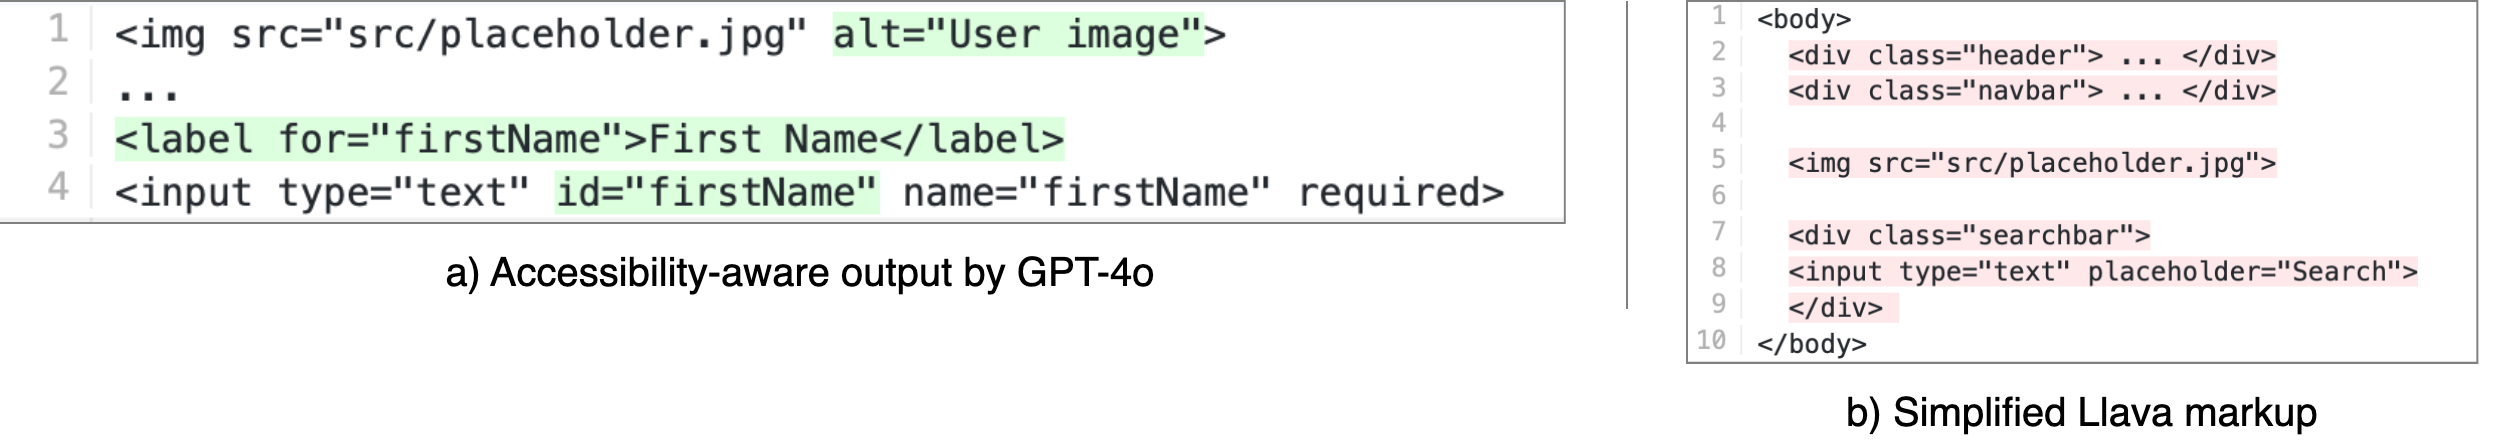
\includegraphics[width=1\linewidth]{figures/generalcapability.png}
  \caption{Comparison of semantically rich (left) and structurally shallow (right) HTML snippets}
  \label{fig:generalcapabilities} 
\end{figure}

\subsubsection{Code Generation Capabilities.} Despite generating
code with fewer violations, the open-source models Qwen and 
Llava do not necessarily produce accessible webpages.
The detailed analysis reveals that these models tend to generate 
simplistic and semantically shallow code snippets. They often 
generate flat layouts or generic tags, such as \texttt{<div>} or \texttt{<span>},
combined with little nesting, styling, or ARIA annotations as default. 
This behavior is illustrated in Figure~\ref{fig:generalcapabilities} (b),
where Llava reduces a multi-component UI layout into a linear 
sequence of \texttt{<div>} elements, following a common template.
This approach leads to fewer accessibility violations
because it lacks problematic elements and therefore reduces the 
surface for potential issues. However, this results in 
structurally incomplete and visually incorrect code, which can be 
seen in significant lower code similarity scores of 70.36\% for Qwen and
50.50\% for Llava, compared to 88.96\% for GPT and 87.12\% for Gemini.
This indicates that the smaller, open-source models fail to capture 
layout fidelity and semantic depth. This finding highlights the 
necessity to balance accessibility evaluation with structural 
quality, because the absence of content can artificially 
reduce the violation metrics.

\begin{center}
\begin{tcolorbox}[colback=black!5!white,colframe=black!75!black,bottom=-0.05pt,top=-0.05pt]
\textit{\textbf{Finding:}} Due to variations in alignment goals (e.g., GPT's accessibility-aware behavior) and training data composition (e.g., Gemini's dependence on framework-derived styles), accessibility violations differ significantly amongst MLLMs. Open-source models, such as Qwen and Llava, tend to produce simplified, under-specified code, which is the main reason why they report fewer violations.
\end{tcolorbox}
\end{center}


\section{RQ3: Does advanced prompt engineering lead to more accessible MLLM-generated
UI code?}
\subsection{Experiment Setup}
While the prior RQs explored the inherent capabilities of MLLMs with naive
prompting, this RQ investigated the prompting strategies' impact 
on the accessibility of the generated code. Prompt engineering has shown 
to be a powerful technique in prior work to improve and influence the 
behavior of LLMs, especially in structured tasks. Therefore, this study 
takes 7 different prompting strategies into account, ranging from 
naive to externally supported techniques. Note that the prompts follow 
the established best practices of prior research~\cite{suh2025accessiblecode, xiao2024interaction2code}.\newline

\begin{figure}
  \centering
  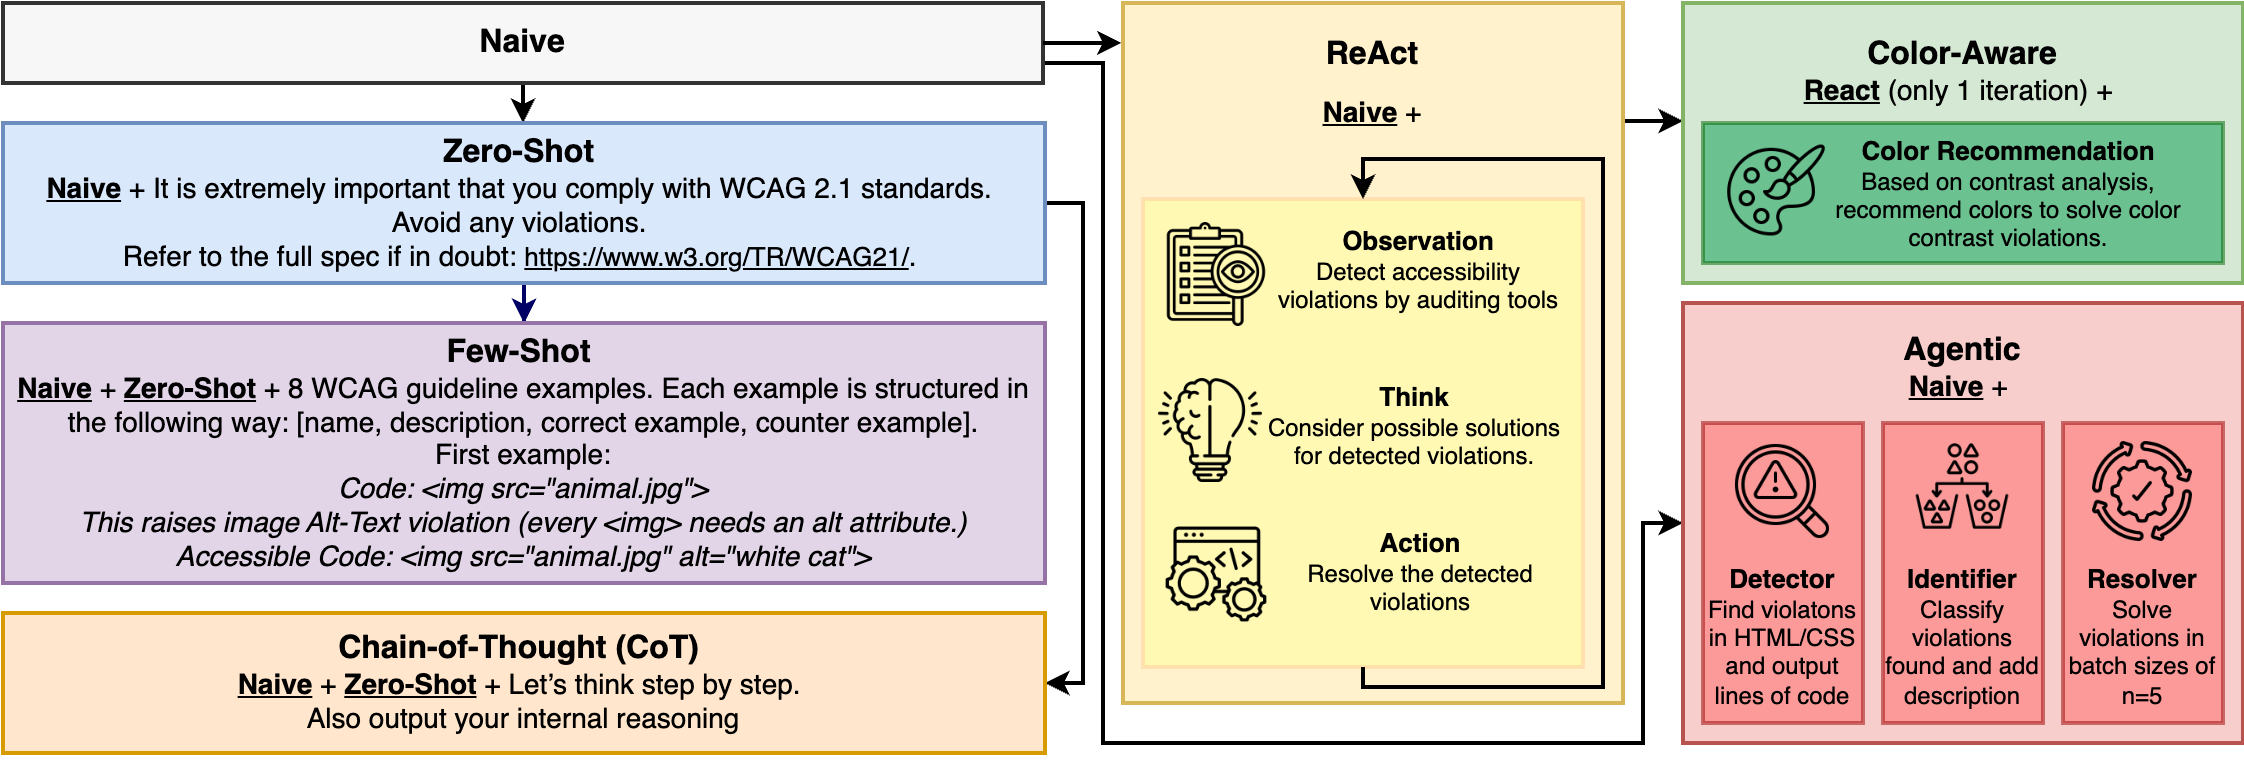
\includegraphics[width=0.85\linewidth]{figures/prompts_new_new.png}
  \caption{Overview of the advanced prompting strategies.}
  \label{fig:prompts_new} 
\end{figure}



\textbf{Naive Prompting (Baseline)}: 
  Without explicit accessibility instructions, the model is
  instructed to generate HTML/CSS code based on a screenshot of a webpage.\newline\newline
\textbf{Zero-Shot Prompting}: 
  The MLLMs are explicitly instructed to 
  generate accessible code by adding the instruction \textit{``comply with WCAG 2.1 standards''}, 
  as shown in Figure~\ref{fig:prompts_new}. 
  This explores the model's ability to generalize accessibility guidelines 
  only based on an instruction and without examples.\newline\newline
\textbf{Few-Shot Prompting}: 
  This strategy resembles the zero-shot prompt,
  but is enriched with several examples of WCAG 2.1 guidelines, combined 
  with a description of the task, an incorrect code snippet, and a 
  corresponding correct code snippet.
  The examples are sourced from the ARIA Authoring Practices Guide 
  (by W3C)~\cite{web:w3c_examples} and Accessible Components by Gov.uk 
  Design System~\cite{web:govuk}, which are known for their accessibility
  best practices.
  Eight examples, which differ in their content (e.g., image alt-text, 
  form labels, landmarks) are manually collected. They serve as an 
  additional context for the model to lead the models towards a more 
  accessible code generation.\newline\newline
\textbf{Chain-of-Thought Prompting}: 
  As shown in Fig.~\ref{fig:prompts_new}, 
  the prompt encourages the model to think step-by-step. 
  The objective is to guide the model to describe its 
  considerations in a structured plan and finally output the code.
  This helps to show intermediate reasoning steps that possibly 
  highlight accessibility-aware thinking.\newline\newline
\textbf{Agentic Prompting}: 
  As prior research~\cite{wu2023autogen} has shown, the use of multi-agent 
  systems, where each agent has a specific task, can lead to better
  results in complex tasks. Therefore, this strategy splits the 
  task of creating accessible code into three agents: The 
  \textit{Detector} agent is designed to detect accessibility violations 
  in a generated code, instructed with the naive prompt. It outputs a list
  of snippets with violations, including their location in the code. The 
  second agent, the \textit{Identifier}, is responsible for classifying 
  the violations into their respective WCAG guidelines (e.g., 
  color contrast, landmarks, etc.) and enrich the each violation with 
  its severity level. The third agent, the \textit{Resolver}, is 
  instructed to resolve the list of violations in the code. In order to 
  prevent cascading errors, this agent is instructed to solve batches 
  of violations, having a size of \(n = 5\). The goal of this strategy 
  is to evaluate whether decomposing the task into smaller and more 
  manageable subtasks can improve the overall accessibility.\newline\newline
\textbf{ReAct Prompting}: 
  This strategy first instructs the model to generate HTML/CSS code, 
  according to the naive prompt and then critique its accessibility
  violations detected by the automated tools. As shown in 
  Fig.~\ref{fig:prompts_new}, the model is then asked to revise
  all violations found, prioritize those with the highest 
  severity and output the revised code.
  This multi-step approach evaluates the capability of the model to 
  self-correct and iteratively apply accessibility standards. 
  Each self-refinement loop runs for three iterations or until 
  no further violations are detected.\newline\newline
\textbf{Color Aware Prompting}: 
  As previous RQs have shown, color contrast violations are a common 
  issue in MLLM-generated code. Due to their mathematical nature, they
  can be difficult to solve. Therefore, this strategy extends the ReAct 
  prompting by adding a color-aware step. It uses a pre-processing 
  step which extracts the color values from the screenshot, analyzes 
  the color contrast violations found and provides the model with a 
  possible solution for each violation. Similar to the ReAct prompting,
  the model is then instructed to output the revised code. 
  By basing the model on extracted color values and recommended 
  replacements that satisfy WCAG thresholds, the objective is to 
  decrease color-contrast accessibility violations. The model is 
  directed to generate code that maintains visual consistency while 
  utilizing compliant color pairs by supplying this analysis and 
  asking for a revision.
  Note that the refinement loop runs only for one iteration.\newline


Note that all prompting techniques are tested on GPT and Gemini by using the 
same benchmark dataset.


\subsection{Results}
Table~\ref{tab:access-viol-models} presents the average number of accessibility 
violations (AV), total violations (TV), code similarity (CodeSim),
inaccessibility rate (IR) and impact weighted inaccessibility rate (IWIR).
The results demonstrate that advanced prompting techniques can significantly
reduce the amount of accessibility issues in the generated code. For instance,
when using the most advanced prompt (ReAct), 95.75\% of the violations for 
GPT and 82.07\% for Gemini are resolved, compared to the naive counterpart.
A similar trend can be observed for the IR and IWIR. While the 
IR is reduced to 0.68\% for GPT and 1.36\% for Gemini using the ReAct 
prompt, the IWIR is reduced to 13.56\% and 21.48\%, respectively. However, 
the effectiveness of each prompting strategy varies across the models and 
some strategies are more suited for certain models than others.


\begingroup
    \begin{table}[htbp]
  \centering
  \footnotesize
  \setlength{\tabcolsep}{2pt}
  \begin{tabular}{l *{2}{ccccc}}
    \toprule
    \multirow{2}{*}{\textbf{Technique}} &
      \multicolumn{5}{c}{\textbf{GPT}} &
      \multicolumn{5}{c}{\textbf{Gemini}} \\
    \cmidrule(lr){2-6}\cmidrule(l){7-11}
      & Average Violations & Total Violations & CodeSim & IR & IWIR
      & Average Violations & Total Violations & CodeSim & IR & IWIR \\
    \midrule
    Naive               & 13.75 & 729 & \underline{\textbf{88.96\%}} & 12.22\% & 47.10\%
                        & 15.45 & 819 & \underline{\textbf{87.12\%}} & 11.42\% & 47.70\% \\
    Zero-Shot           & 12.33 & 653 & 87.79\% & \textemdash & \textemdash
                        & 14.25 & 755 & 86.85\% & \textemdash & \textemdash \\
    Few-Shot            &  9.49 & 503 & 87.29\% & \textemdash & \textemdash
                        & 15.74 & 834 & 86.95\% & \textemdash & \textemdash \\
    Chain-of-Thought    & 10.04 & 532 & 87.91\% & \textemdash & \textemdash
                        & 14.28 & 757 & 86.80\% & \textemdash & \textemdash \\
    ReAct               & \underline{\textbf{0.68}} & \underline{\textbf{36}} & 86.94\% & \textemdash & \textemdash
                        & \underline{\textbf{2.77}} & \underline{\textbf{147}} & 86.16\% & \textemdash & \textemdash \\
    Color-Aware         & \textemdash & \textemdash & \textemdash & \textemdash & \textemdash
                        & \textemdash & \textemdash & \textemdash & \textemdash & \textemdash \\
    Agentic             & \textemdash & \textemdash & \textemdash & \textemdash & \textemdash
                        & \textemdash & \textemdash & \textemdash & \textemdash & \textemdash \\
    \bottomrule
  \end{tabular}
  \caption{Performance for advanced prompting techniques (including IR and IWIR).}
  \label{tab:access-viol-models}
\end{table}

\endgroup

\subsubsection{Impact of Zero-Shot Prompting}
All models show a moderate, but measurable improvement in accessibility 
violations when a simple instruction about accessibility is added to 
the prompt. For instance, GPT reduces the average amount of 
violations by 10.33\% and Gemini by 7.76\%, compared to the 
naive prompt. However, while the IR shows a similar trend with 
a considerable reduction for both models, the IWIR remains almost 
unchanged, even showing a slight increase. This suggests that even 
if the models are capable of activating their accessibility 
awareness, even without explicit examples, they still struggle to 
solve the most severe violations.\newline
A deeper analysis of the violation types and their distribution 
reveals that some limitations for the models remain. For example,
both models often use accessibility-related attributes (e.g., 
label, alt, role, aria-*) but misuse them and fail to apply them 
in a consistent manner. Figure~\ref{fig:zero-shot-example} demonstrates
a representative example. While Gemini generates an e-mail 
subscription form field, it fails to provide any accessible name,
e.g, neither a \texttt{<label>} nor an \texttt{aria-label} attribute.
This indicates that zero-shot prompting triggers awareness, it 
does not necessarily resolve accessibility gaps and inconsistencies.


\begin{figure}
  \centering
  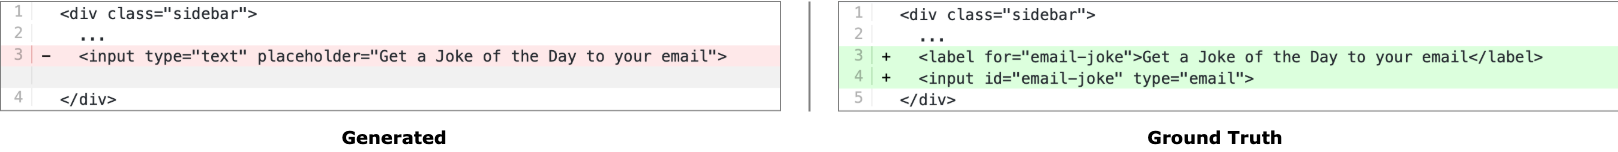
\includegraphics[width=1\linewidth]{figures/zeroshot-example.png}
  \caption{Failure example for zero-shot prompting.}
  \label{fig:zero-shot-example} 
\end{figure}

\subsubsection{Impact of Few-Shot Prompting}
The few-shot prompting technique results in a 30.98\% improvement
in accessibility performance for GPT, with the average number 
of violations dropping from 13.75 to 9.49 and the IR 
decreasing from 12.22\% to 7.96\%. By observing 8 
high-quality, concrete examples, the model is capable of 
copying the underlying patterns and structure. For instance,
when provided with an example of correct heading structures, such 
as \texttt{<h1>}, GPT is able to incorporate this pattern into its
generation, reducing the average number of heading violations 
from 26 to 15. Furthermore, the examples presented 
reflect important accessibility guidelines, having a 
significant impact on users and therefore also a high 
severity. This is reflected in the IR, which drops from 
47.10\% to 44.64\%.
This demonstrates the importance of concrete 
examples in guiding the model, especially for concepts like
accessibility, which may be underrepresented in the training data.\newline
However, surprisingly Gemini does not show similar improvements, in fact, 
it performs slightly worse with an increase of 1.88\% in the average
number of violations. Based on the qualitative analysis, this 
effect can be attributed to two primary factors. First, Gemini 
exhibits a 56.52\% increase in violations related to the 
\emph{Distinguishable Links} category. Due to its exposure 
to link-related examples, it tends to generate links more 
frequently, but often without sufficient contrast or 
styling, violating the WCAG requirements. This phenomenon 
may be directly linked to the color bias in the training data,
which has been observed in RQ2. Gemini tends to use generic, default 
colors and links, such as the primary blue from the Bootstrap framework,
that is used as the main color for links. This leads to 
a lack of distinction between links and the body text.\newline
The second violation category 
\emph{Landmark \& Region} increases by 12.83\%, due to 
Gemini's tendency to misuse the semantic 
elements, such as \texttt{<main>} or \texttt{<nav>}. This 
can likely be attributed to a misinterpretation of 
the few-shot examples, which might be replicated 
directly without deeper semantic understanding in 
how those elements contribute to accessibility.

\subsubsection{Impact of Chain-of-Thought Prompting}
Chain-of-Thought prompting results in notable improvements 
over the naive prompt, i.e., averaging 10.04 vs 13.75 violations
per UI for GPT and 14.28 vs 15.45 for Gemini. Due to 
the reasoning instruction before generating code, 
the models are able to reflect possible accessibility 
constaints often missed in direct code generation.
Interestingly, GPT benefits significantly more 
than Gemini, with a relative improvement of 26.98\% vs 
7.57\%. This is probably due to the fact that GPT constantly 
outlines an organized structure to reasoning by 
recognizing particular accessibility issues 
(such as contrast ratios and alt text) and integrating them into 
the code that is generated. In contrast, Gemini's 
CoT reasoning is less consistent and frequently omits 
key steps or fails to use the reasoning effectively 
during code generation.

\subsubsection{Impact of Agentic Prompting}
Splitting the task into three agents only leads to 
moderate improvements, as GPT reduces its violations 
by 17.53\% and Gemini by 14.82\% compared to the naive 
baseline. Similar to the prior strategies, the IR follows 
the same trend, dropping from 12.22\% to 8.86\% for GPT and
from 11.42\% to 8.36\% for Gemini, but the IWIR decreases much less
with 11.25\% for GPT and only 1.47\% for Gemini.\newline
The qualitative analysis reveals two main reasons for these 
results. First, the \textit{Detector} agent misses some 
violations in the generated code and occasionally even reports 
false positives. As a result, the \textit{Resolver} agent 
either does not resolve all violations within the code 
or changes already correct markup, which leads to new 
violations. Second, the resolver resolves the violations in 
batch sizes. This can prevent the Resolver in understanding 
layout dependencies, leading to small, but significant changes 
that decrease the layout fidelity which results in the 
lowest code similarity of all prompting techniques
(86.12\% for GPT and 85.07\% for Gemini). In general, 
while the agentic prompting reduces the load per step of 
the models, it introduces additional noise which 
propagates through the agents.

\subsubsection{Impact of ReAct Prompting}
The experiment shows that both GPT and Gemini significantly 
improve their accessibility performance when using the ReAct 
prompting strategy. Across three iterative refinement 
cycles, GPT achieves reductions of 82.33\%, 92.07\% and 95.05\% 
in accessibility violations compared to the naive prompt, while 
Gemini improved by 62.14\%, 77.67\% and 82.07\%, respectively.
Similar improvements can be observed for the IR and IWIR. 
After 3 iterations, only 0.44\% of nodes in GPT's code
contain accessibility violations, while Gemini has an IR of 1.36\%.
Interestingly, not only the amount of violations, but also 
their severity is reduced. For instance the IWIR drops from 
47.10\% to 13.56\% for GPT and from 47.70\% to 21.48\% for Gemini.
This indicates that the model is not only capable of 
resolving violations, but also prioritizes the violations 
with severity \emph{serious} or \emph{critical}. After 3 
refinement iterations, neither GPT nor Gemini produces 
any violations with severity \emph{critical} and only 
few with \emph{serious}.\newline 
The results suggest that even if models not inherently 
obey all accessibility guidelines, they can be
guided towards more accessible code by incorporating 
external observations of the automated tools. GPT 
consistently outperforms Gemini across all iterations,
possibly due to its stronger alignment with 
Reinforcement Learning from Human Feedback (RLHF) which 
equips it with a better capacity to self-correct and 
obey instructions based on user-oriented feedback.\newline 
A notable observation from the ReAct prompting is that the 
two main categories of accessibility violations, 
color contrast and landmarks, are significantly reduced.
While landmark violations are reduced by 98.21\% for GPT and
95.85\% for Gemini, color contrast violations are reduced by
90.58\% and 64.93\%, respectively. 
These results reflect a growing capacity of MLLMs 
to add feedback into their stylistic choices, which 
leads to more accessible and visually consistent webpages.\newline 
However, also the ReAct prompting has its limitations.
Even though, both 
models decrease the dependency on framework-based 
colors, the results still 
vary across the models. For instance, especially 
during the first refinement iterations, Gemini still 
heavily relies on framework-based color palettes, 
especially, Bootstrap's primary blue, which leads to 
an increase in those violations of 23\% with 
this exact color, even though overall the amount 
of color contrast violations is reduced by 22\%. 
This suggests that the model might not be able to 
synthesize its own new colors, but rather tries to
substitute problematic colors with known colors 
from its training data.
Furthermore, some
attempts to fix particular violations can 
occasionally lead to new problems elsewhere in 
the code. As Fig~\ref{fig:iterativecascadingissues} suggests, the model 
successfully solves certain violations (for example adds 
a \texttt{label} to the form element), but at the same time 
introduces a new issue with the color contrast of the label.
These cascading error may arise from a limited 
understanding of the codes underlying structure and 
dependencies, which highlights a potential limitation 
of current MLLMs.

\begin{figure}
  \centering
  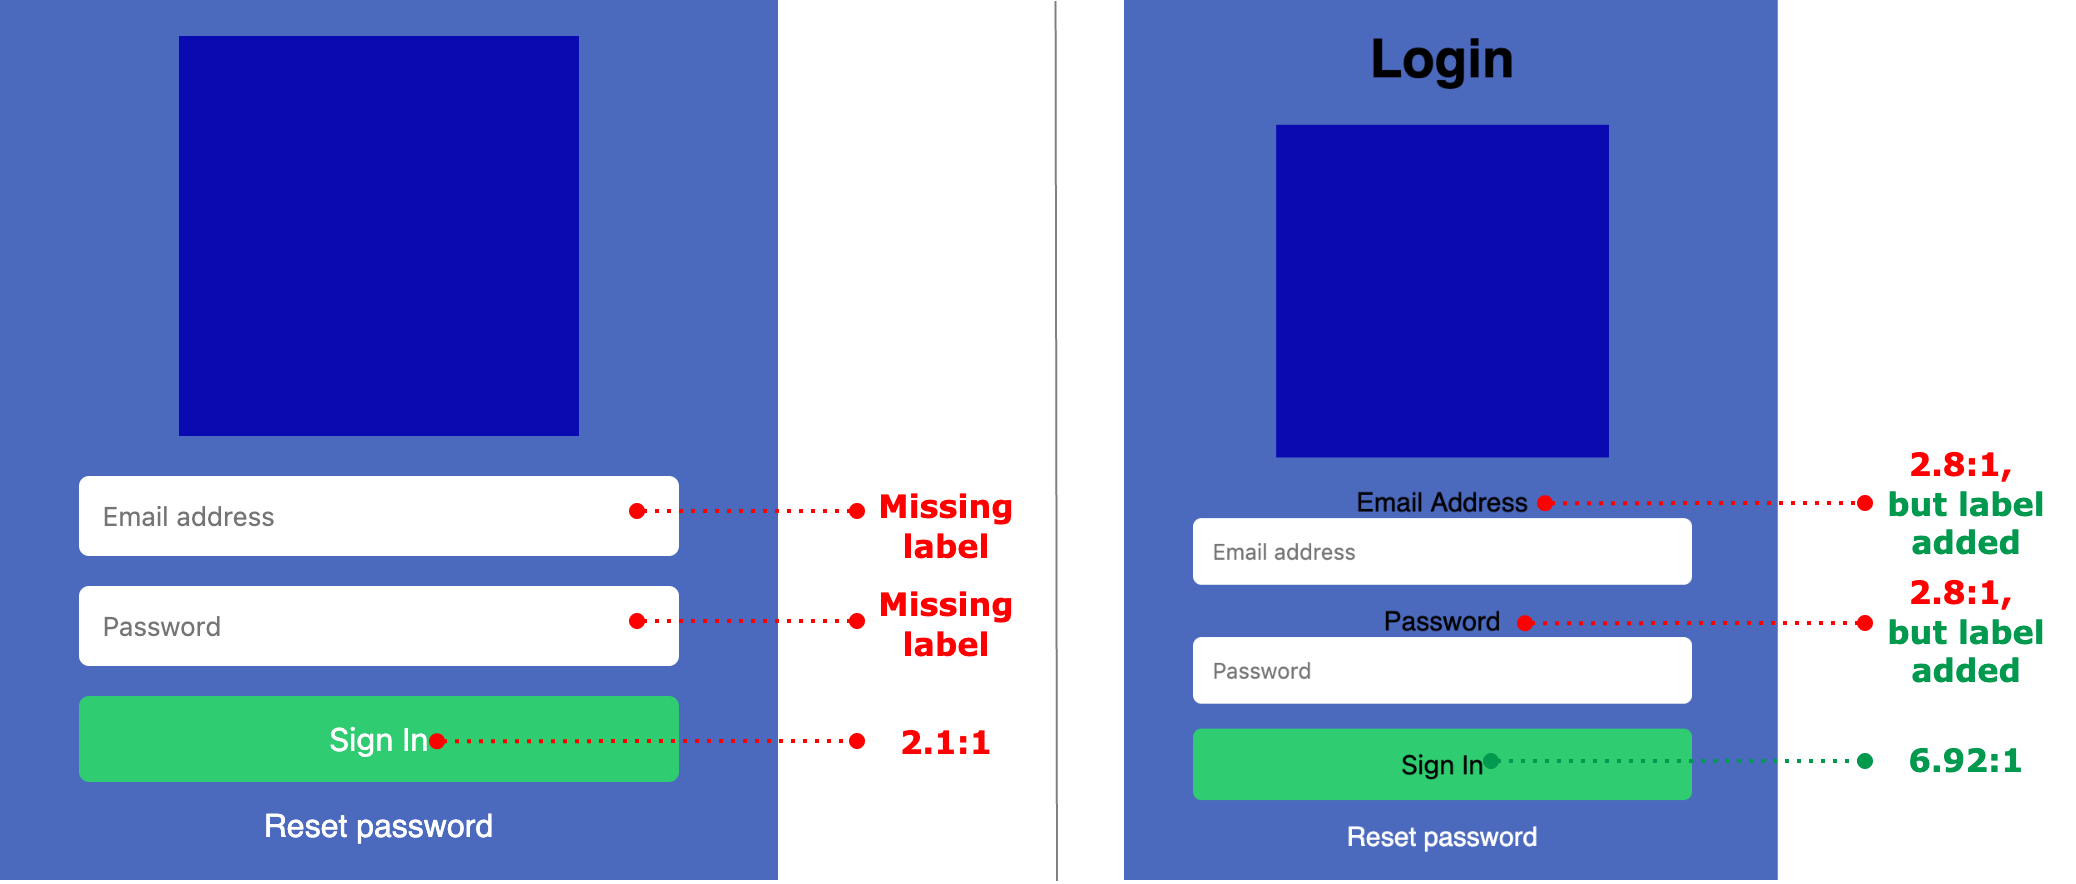
\includegraphics[width=0.9\linewidth]{figures/iterativecascadingissues.png}
  \caption{Login screen before (left) and after (right) the first refinement iteration. The model successfully solves the missing label violation, but introduces a new issue with the color contrast of the label.}
  \label{fig:iterativecascadingissues} 
\end{figure}

\subsubsection{Impact of Color-Aware Prompting}
Enhancing the ReAct prompting technique with pre-computed 
and WCAG-compliant colors has a different impact on both models.
While Gemini struggles to invent new colors, it 
benefits the most with its average number of violations 
dropping by 83.30\%, compared to the naive prompt and 
is even able to reduce its number by 6.86\%, compared to 
the ReAct prompting. While GPT also benefits from this 
strategy, by reducing its violations by 75.64\%, it does not
match the improvements of the ReAct prompting strategy.\newline
Two main reasons can be attrubuted to this finding. First,
GPT is already able to synthesize new colors. Providing 
new externally computed colors, occassionally leads to 
conflicts elsewhere in the code, as the model tries to 
incorporate these colors. Second, the bounding-box 
detection of \textit{Design2Code} occasionally groups elements
together that are not visually connected in the UI. This 
can lead to situations where the model applies external 
colors for an entire region, rather than the specific node.
Overall, the results suggest that adding explicit WCAG-compliant 
colors can significantly lower contrast violations. However, 
the underlying model's design capabilities and accuracy 
determines how beneficial this strategy is.


\begin{center}
\begin{tcolorbox}[colback=black!5!white,colframe=black!75!black,bottom=-0.05pt,top=-0.05pt]
\textit{\textbf{Finding:}} Prompting strategies significantly 
influence the accessibility of MLLM-generated UI code. 
While the models benefit from explicit guidance, 
advanced techniques like ReAct prompting yield the most 
substantial improvements. However, each strategy may also 
introduce model-specific limitations and, in some cases, 
create new issues. These findings underscore the importance 
of aligning prompting strategies with model capabilities 
to enhance accessibility outcomes.
\end{tcolorbox}
\end{center}


\section{RQ4: How consistent are the accessibility violations across different MLLMs on the same UI screenshot?}
\subsection{Experiment Setup}
The objective of this RQ is find out wether different MLLMs 
cause similar or complementary accessibility violations when 
asked to generate HTML/CSS from the same UI screenshot.
Consistent error patterns would indicate that systematic 
limitations, caused by a similar training data, exist. 
In contrast, complementary violations would motivate 
ensemble or shared approaches between the models to improve the 
overall accessibility of the generated code.
To investigate this, the benchmark dataset is used, which 
is prompted to GPT-4o and Gemini-2.0 flash with 
the naive prompting technique. For every tuple of
screenshot and model, the list of accessibility violations
is extracted, sorted and represented by a violation 
vector, which counts the number of issues per 
WCAG class. 



\newcommand{\vect}[1]{\begin{pmatrix}#1\end{pmatrix}}
\newcommand{\issues}{k}                   % Anzahl der Issue-Klassen
\newcommand{\vx}{\mathbf x}
\newcommand{\vy}{\mathbf y}

\textbf{Violation Vectors:}  
  For each tuple of screenshot and model, the number of violations per class is counted as follows:
  \[
  \left(
    \begin{array}{@{}l r@{}}
      \text{Issue}_{1}: & x_{1}\\
      \text{Issue}_{2}: & x_{2}\\
      \vdots           & \vdots\\
      \text{Issue}_{\issues}: & x_{\issues}
    \end{array}
  \right)
  \xmapsto{\text{to vector}}
  \mathbf v \;:=\;
  \vect{x_{1}\\x_{2}\\\vdots\\x_{\issues}} \in \mathbb R^{\issues}.
\]

To compare the similarity of the violation vectors, the 
cosine similarity is used, which is common metric in 
other research areas. 

\textbf{Cosine Similarity}  
  Given two vectors with $\vx,\vy\in\mathbb R^{\issues}$, the cosine similarity is defined as:
  \[
  \operatorname{cos\_sim}(\mathbf v_1,\mathbf v_2)=
  \frac{\mathbf v_1^{\mathsf T}\mathbf v_2}{\lVert \mathbf v_1\rVert\,\lVert \mathbf v_2\rVert}
  \quad\in[0,1].
\]


\subsection{Results}
Figure~\ref{fig:cosinesimilarity} shows the cosine similarity matrix 
plotted as a heatmap, where each cell represents the similarity between 
the violation vectors of different model runs. 
As the figure shows, the majority of the cells 
are light-colored, indicating a high cosine similarity 
between the runs of the models. This is especially true 
for the upper part of the heatmap, representing the 
dataset entries of the Design2Code dataset, reaching 
from example 1 to 28. In this section, the models 
show a high degree of consistency and similarity, across 
both models, but also across the individual runs.
The lower part of the heatmap, representing the
dataset entries from the dataset Webcode2m, show 
a more diverse pattern, with a mix of lighter and 
darker cells. Nevertheless, also in this section, 
the majority of the cells are light-colored, showing
that the models are still consistent in their violation 
patterns. A manual inspection of the darker cells reveals 
that a great number of lower similarity scores stems from 
two main reasons: 1) In some runs, a model is capable 
to generate code with only few violations, leading to 
a violation vector with many zeros or small values. 
Even if the other model achieves to generate code 
which has a relatively low number of violations too, 
the cosine similarity is highly sensitive to 
small values, which leads to a low similarity score. 
This is especially true for the section which stems from 
the Webcode2m dataset, where the models are able to
generate code with fewer violations. 
2) The second reason for lower similarity scores stems 
from possible cascading errors in the code generation. 
For instance, if one model generates a code snippet with
a color palette that is not compliant with WCAG, it 
is likely that the amount of color contrast violations 
in this snippet is higher than in other runs which 
might use a different and better color palette. 
This can lead to a lower cosine similarity score, even
if the other violations are similar.\newline 
Overall, the results suggest that the models generate 
code snippets with similar amounts of accessibility violations
and error distributions. The high similarity score 
indicates that the models are likely to share similar
limitations and biases, which can be attributed to the
underlying training data.

\begin{center}
\begin{tcolorbox}[colback=black!5!white,colframe=black!75!black,bottom=-0.05pt,top=-0.05pt]
\textit{\textbf{Finding:}} Accessibility violations 
are highly consistent across GPT and Gemini, with an 
average cosine similarity of 0.719. This suggests that 
the models inherit the same systemic blind spots from 
web-scale training data.
\end{tcolorbox}
\end{center}


\begin{figure}
  \centering
  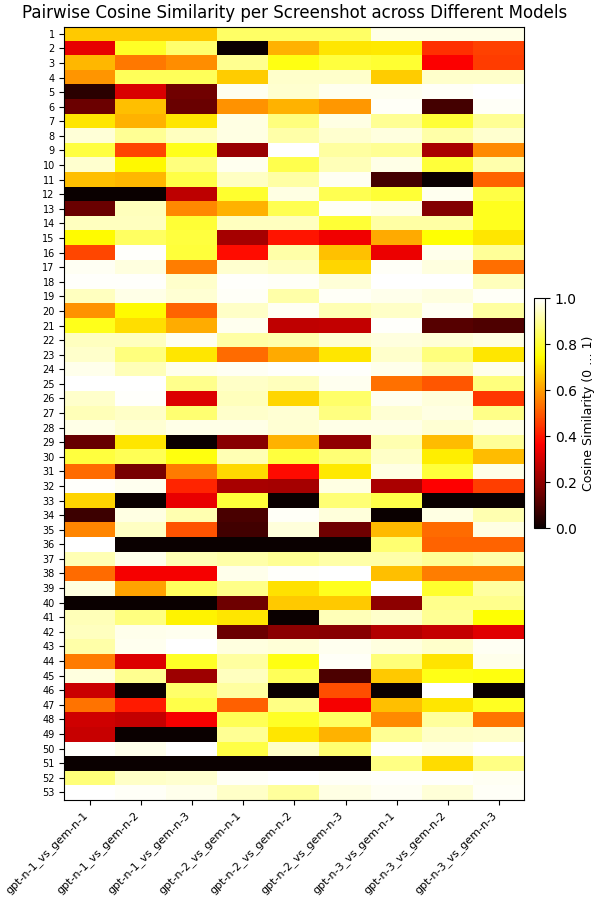
\includegraphics[width=0.4\linewidth]{figures/cosinesim.png}
  \caption{Cosine similarity heatmap between the 3 runs of GPT and Gemini on the same UI screenshot. 
  Each cell represents the cosine similarity of the accessibility violation vectors generated by the models.
  Light = high similarity, dark = low similarity.}
  \label{fig:cosinesimilarity} 
\end{figure}





\section{RQ5: Does data leakage affect the accessibility of MLLM-generated UI code?}
\subsection{Experiment Setup}
A concern that is often raised in the context of MLLMs is 
the possibility of data leakage, where the models have 
already been exposed to the test data during pretraining, 
thus leading to inflated performance. This RQ aims to 
investigate whether such leakage has an impact on the
the accessibility of the generated code.\newline
To investigate this, 2 distinct datasets have been created 
in order to compare model performance. 1) \textbf{Benchmark Dataset},
which has been used and described in the previous RQs. 2)
\textbf{Synthetic Dataset}, consists of two distinct 
subsets. The first subset is
created with layout mutation and 
hybrid synthesis techniques. This subset contains new 
UI compositions and code which is not likely to have 
exact matches in the pretraining data. Therefore, 
heuristic transformation rules have been created to 
mutate layout structures, elements arragements,
component colors and text content. In a second step,
some layouts and components are then interchanged across 
the UIs, which leads to new compositions. An example 
of this synthetic dataset is shown in Fig.~\ref{fig:dataleakagemutation}.
As a result, 10 webpages are synthesized, which are 
rendered into screenshots and paired with their 
corresponding mutated HTML/CSS code. 
The second subset is created to complement 
more up-to-date and real-world examples in the synthetic 
dataset. This subset is curated by selecting two 
open-source web projects~\cite{web:alphaonelabsedu, web:ecommerceferhan}
that are created after the official knowledge cutoff 
dates of the MLLMs. These projects contain new samples 
that are unlikely to have been seen during pretraining.
However, web code from open repositories often 
includes dynamically generated content, external dependencies 
and redundant content, which can bias this accessibility-focused 
analysis negatively. Therefore, the collected code 
is manually cleaned according to the previous 
steps, described in Section~\ref{subchapter:Dataset}.
Through this process, 10 new webpages are collected and
their corresponding HTML/CSS and rendered UI screenshots 
are added to the subset.\newline
The two subsets are then combined into a single 
synthetic dataset, which is used to compare the 
models' performance against the benchmark dataset.\newline
All experiments use the same naive prompting setup 
and are conducted on GPT-4o and Gemini-2.0 flash. 
By comparing the code similarity and distribution of 
accessibility violations across the 
different datasets, it can be evaluated 
whether the performance variations suggest
memorization or data leakage effects.

\begin{figure}
  \centering
  \includegraphics[width=0.9\linewidth]{figures/dataleakage.png}
  \caption{Original web page (left), a heuristically mutated version (middle) with altered colour, layout and text, and a cross-site hybrid combining sections from multiple pages (right). May get drawing inspiration from this paper: GUIGAN: Learning to Generate GUI Designs Using Generative Adversarial Networks}
  \label{fig:dataleakagemutation} 
\end{figure}

\begingroup
    \begin{table}[htbp]
  \centering
  \small
  \setlength{\tabcolsep}{2pt}
  \begin{tabular}{l
                ccc            % GPT columns
                @{\hspace{10pt}}
                ccc}           % Gemini columns
    \toprule
    \multirow{2}{*}{\textbf{Dataset}} &
      \multicolumn{3}{c}{\textbf{GPT}} &
      \multicolumn{3}{c}{\textbf{Gemini}} \\
    \cmidrule(lr){2-4}\cmidrule(l){5-7}
      & CodeSim & IR & IWIR
      & CodeSim & IR & IWIR \\
    \midrule
    Benchmark & 88.96\% & 12.22\% & 47.10\%
              & 87.12\% & 11.42\% & 47.70\% \\
    Synthetic & 89.17\% & 11.64\% & 49.47\%
              & 88.01\% & 12.06\% & 50.30\% \\
    \bottomrule
  \end{tabular}
  \caption{Code similarity (CodeSim) and accessibility metrics (IR, IWIR) on the Benchmark and Synthetic datasets.}
  \label{tab:dataleakage}
\end{table}

\endgroup

\subsection{Results}
Table~\ref{tab:dataleakage} shows the results across all 
three datasets. Overall, the code similarity scores are 
relatively consistent across the datasets, even showing slightly 
higher values for the synthetic dataset. While GPT 
achieves a code similarity of 88.96\% for the benchmark dataset vs 
89.17\% for the synthetic dataset, Gemini
achieves 87.12\% vs 88.01\%, respectively. This 
suggests that the models are not merely memorizing and 
reproducing the training data, but rather are 
able to generalize and synthesize new code. The 
IR changes by 0.5-0.6 percentage points (GPT 
slightly lower, Gemini slightly higher), which is 
considered within the variance of the models 
shown in RQ3. This indicates that the number of 
DOM nodes with at least one accessibility violation 
is largely unaffected by the underlying dataset.
Lastly, both models show a modest increase in the 
IWIR, with GPT increasing from 47.10\% to 49.47\% 
and Gemini from 47.70\% to 50.30\%. Manual inspection 
reveals that the synthetic dataset, especially 
the 10 mutated UIs, contain more composite sections, 
which tend to trigger slightly more color 
contrast violations, and therefore lead 
to a higher IWIR.\newline
These findings demonstrate comparable performances 
in both code fidelity and accessibility metrics across
the different datasets. This suggests that the results 
shown in previous RQs are not artificially inflated 
by data leakage, but rather reflect the overall 
generalization capabilities of the models. Therefore,
it can be concluded that data leakage is unlikely to 
exist or affect the evaluation process of MLLMs in 
this thesis.

\begin{center}
\begin{tcolorbox}[colback=black!5!white,colframe=black!75!black,bottom=-0.05pt,top=-0.05pt]
\textit{Finding:} The consistent performance of 
MLLMs across the benchmark and synthetic datasets 
suggests that data leakage is minimal 
and the models' behavior observed in earlier 
experiments is not an artifact of memorization 
or pretraining exposure.
\end{tcolorbox}
\end{center}